%
% Draft  document histcollwrin.tex
% Looks at how collagen in Merino sheep skin relates to skin wrinkle and follicle curvature 
%
 
\documentclass[titlepage]{article}  % Latex2e
\usepackage{graphicx,lscape,subfigure}
\usepackage{tikz}
\usepackage{bm,longtable}
\usepackage{textcomp}
 

\title{Histology of collagen in Merino sheep skin and its association with skin wrinkle formation and follicle curvature }
\author{The late J.E. Watts S. Maleki, P.G. Swan, J. Gordon, and N. Jackson}
\date{10 June 2019} 

 
\begin{document} 


 
\maketitle      

$\newcommand{\E}{\mathrm{E}}$
$\newcommand{\Var}{\mathrm{Var}}$
$\newcommand{\Cov}{\mathrm{Cov}}$ 
$\newcommand{\SD}{\mathrm{SD}}$ 

\section{Introduction} 

Wrinkle formation in Australian Merino sheep skin is a phenomenon with serious economic and political consequences.  It has long been known (Seddon, Belschner, and Mulhearn (1931)~\cite{sedd:31}) that wrinkled sheep are more susceptible to blowfly strike. The use of the {\em mulesing} operation to control flystrike in Merino sheep has recently been the subject of intense animal ethics scrutiny, and no effective alternative management option has appeared.
The most effective long term solution would seem to be to breed the wrinkle out of Merino sheep. This has met with resistance from some Australian Merino breeders who feel that the extra skin surface area of wrinkled sheep is necessary to achieve high levels of wool production. Breeding plans which include some culling on wrinkle usually do not lead to its complete elimination (for example Turner Dolling and Kennedy (1970)~\cite{turn:68}).

This study  is an attempt to go back to the basic biology of wrinkle formation, to see whether we can understand the structure of a wrinkle, and to see if that leads to a better approach breeding of wrinkle-free sheep  without lowering productivity or adversely affecting wool quality. 

There have been very few attempts to define what a wrinkle actually is. The early work of Carter(1943)~\cite{cart:43} went as far as describing and naming all the folds on the neck, body, and breech, and developed a set of photographic scores for degree of wrinkle. Carter used the terms {\em fold} and {\em wrinkle} interchangeably, but he distinguished the small {\em pin wrinkles} present in all Merinos, from the larger folds which develop to varying degrees as the sheep matures. From this early start, there is, somewhat surprisingly, nothing on the biology of wrinkles, until the study of Mitchell etal(1984)~\cite{mitch:84}. 

The Mitchell etal(1984)~\cite{mitch:84} paper defines five tissue layers in sheep skin - epidermis, papillary dermis, reticular dermis, layer 4 containing muscle, collagen and elastin, and adipose tissue. These are illustrated in Figure ~\ref{fig:mitchell}
%\documentclass{article}
%\usepackage{graphicx,subfigure}
%\begin{document}

\begin{figure}[!h]
  \centering
  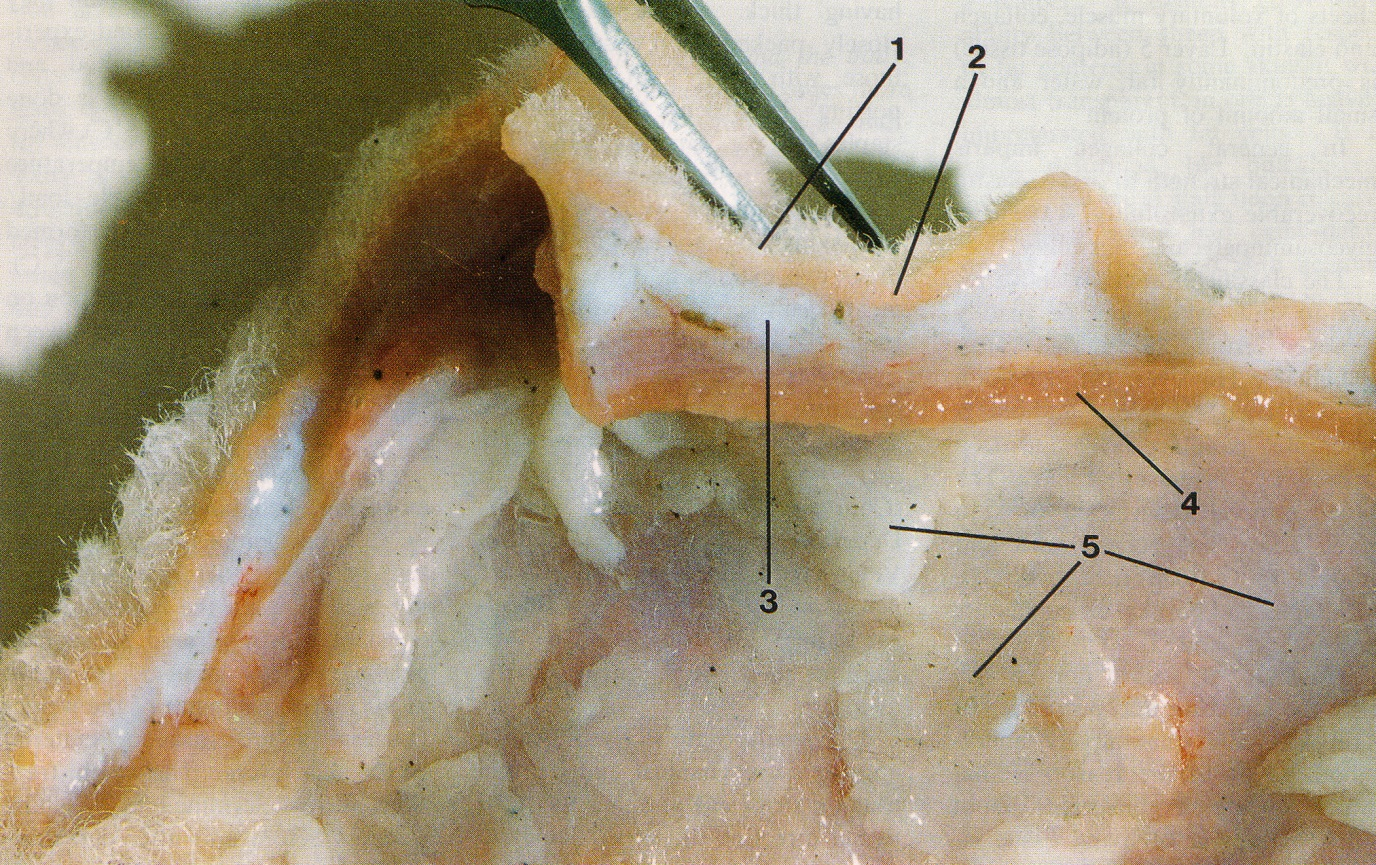
\includegraphics[width=1.0\textwidth]{sanazcollagenwrinkle-img1.jpg}
  \caption{Merino sheep skin showing layers. 1. epidermis with wool fibres; 2. papillary layer of dermis; 3. reticular layer of dermis; 4. areolar tissue and muscle; and 5. adipose tissue. Two wrinkles are present; one alongside each side of the forceps (from Mitchell et al (1984)~\cite{mitc:84})}
  \label{fig:mitchell}
\end{figure}

%\end{document}


Only the first 3 layers curve upward in a folded section of skin, layers 4 and 5 remain straight. This can be seen in Figure ~\ref{fig:mitchell}. Mitchell etalshowed that if layers 4 and 5 were removed, then the folded sections relaxed and flattenned. The implication is that the first 3 layers in a fold are longer then the underlying layers so that the collagen binding layer 4 holds the upper 3 layers in the curved or folded shape.

We refer to the Introduction section of the Jackson and Watts(2017)~\cite{jack:17b} document, where we review the place of wrinkle or skin folds in Merino breeding, and where we specifically refer to the suggestion that all skin wrinkle must be culled from a sheep flock, before they can be successfully selected for the SRS-Merino breeding criteria. This statement leads to the questions of when and how wrinkle development interferes with follicle development to such an extent that breeding of superior Merinos using SRS methodology should be impossible in the presence of wrinkle. An attempt was made , in Jackson and Watts(2017)~\cite{jack:17b} to put forward the hypothesis that wrinkles form in the foetus at the same stage as secondary follicle development so would be likely to affect secondary follicle density or S/P ratio or secondary fibre diameter. This was based on a somewhat obsure reference (Bogolyubsky (1940)~\cite{bogo:40}) which asserts that wrinkles were observed forming in foetal skin of Karakul and Merino lambs at around 100 days of gestation. There are no other studies of wrinkle development, but there is a considerable literature on follicle development ( see Fraser and Short(1960)~\cite{fras:60} and Maddocks and Jackson(1988)~\cite{madd:88} and Ryder and Stevenson(1968)~\cite{ryde:68} for reviews). There is some literature on collagen development in sheep skin, and we will look at that below.

What is proposed here is that the amount and type ( and maybe timing and arrangement in the skin) of collagen development might be a common factor involved with both wrinkle development and follicle development. So what is known about collagen? Well, it is already there in the foetal skin at the time follicles develop (Knight et al (1993) ~\cite{knig:93}).  These authors distinguish two collagen types ( Type III or 'soft' collagen, and Type I or 'hard' collagen) and note  that Type III is highest at 75 days of gestation, and falls progressively as the foetus develops, while Type I is low at day 75 and rises to over 50 percent by birth. Collagen fibres are formed from cells called {\em fibroblasts}. At 75-80 days the fibroblasts appear as plump, immature cells surrounded by reticular collagen fibres which are composed of Type III collagen. By birth the fibroblasts have matured  and the collagen fibres may be intermeshed to varying degrees. If the fine reticular fibre pattern remains, it is soft collagen, if the fibres intermesh the collagen tissue is hardened to various degrees. 

The arrangement (location) of collagen in the skin is also important. In adult skin, Mitchell(1984)~\cite{mitc:84} distinguishes 5 layers in a vertical section of sheep skin
\begin{description}
\item[Layer1] epidermis is mainly keratinised protein
\item[Layer2] contains wool follicles and accessory glands, and is part of the dermis. Sometimes called {\em papillary layer}.
\item[Layer3] layers 2 and 3 together called 'dermis' . Contains fibrous proteins, collagen, and elastin. Sometimes called {\em reticular layer} although the structure is not always reticular, but may be interwoven.
\item[Layer4] contains volunntary muscle, collagen and elastin
\item[Layer5] fat tissue
\end{description}
Mitchell notes that Layer2 is much weaker than Layer 3 ( collagen not as hard). When wrinkles or folds occur in the skin, Layers 1,2, and 3 buckle up into a fold, while Layers 4-5 are straight. It appears as if wrinkles are formed either by an overgrowth of Layers 1-3, or by a shrinkage or tightening of Layer 4. Mitchell has demonstrated this conclusively by showing that if Layer4 (and Layer 5) are dissected away from a skin specimen with wrinkles, the folds in Layers 1-3 flatten out. So in a wrinkled sheep, Layer 4 is holding the skin under some tension, which relaxes when Layer 4 is removed.

So there is some link between collagen development in the skin, and wrinkle formation. If the collagen grows unevenly across the boundary between Layers 3 and 4, the top 3 layers form a fold to accomodate. Since wrinkles mostly form in rows, this unevenness of collagen development must be in one dimension - if it were 2 dimensional the upper 3 layers of skin would form a lump, rather than a fold. There is no reported observation of directional unevenness of collagen across Layers 3/4, but it must be so, or we would get lumps rather than folds.

We need to also ask if there are links between collagen development and follicle development. 

\section{Materials and Methods}
\subsection{Sheep studied}
This is a small study. A total of 106 sheep, representing fine, medium, and strong wool strains of Merino, were sampled from 5 flocks over the period 1988 to 2003. The flocks and sheep were chosen to ensure that all four grades of  SkinType (as defined by Watts et al (2017)~\cite{watt:17}) were well represented. The four SkinType grades contain information on skin wrinkle, but are not wrinkle alone.

\subsection{Measurements}
The following measurements and scores were available
\begin{description}
\item[SkinType] visual scores for sheep skin type. Four grades SRS, semi-SRS, flat, and tight, as defined by Watts et al (2017)~\cite{watt:17}.
\item[TST] total skin thickness in mm. Measured with a ruler graduate in 0.1 mm divisions at 3x magnification on the midside skin sample trimmed of wool stuble and subdermal fat. It consists of epidermis, papillary layer, and reticular layer (layers 1 to 3).
\item[CST] compressed skin thickness in mm. Measured on the trimmed sample with a Mitutoyo ballpoint depth guage ( graduated in 0.1 mm divisions) at four sites. Analyses are of the mean CST over 4 sites.
\item[CMP] compressibility as a percentage. Calculated from CST and TST as $CMP = 100(TST-CST)/TST$. Measures the reduction in thickness under compression as a percentage of the uncompressed thickness.
\item[SkinSoft] skin softness score or ease with which the skin bends or buckles. Five grades (1=hard, unable to bend), to (5=supple, bends easily). Assessed by manually bending the trimmed skin sample in two directions ( north-south = across the rows of follicle groups) and (east-west = along the rows of follicle groups).
\item[S/P] ratio of secondary to primary follicle numbers. This ratio is normally used as a measure of secondary follicle density which is independent of skin expansion during growth. Measured on skin sections.
\item[Fn] follicle number per unit area in follicles per $mm^{2}$. Measured on skin sections with a correction for shrinkage during processing
\item[Dp] mean fibre diameter of secondary fibres in $\mu m$. Measured on skin sections.
\item[DpSD] standard deviation of secondary fibre diameters in $\mu m$. Measured on skin sections.
\end{description}

\subsection{Interpretation of measurements}
Some care is needed in defining what these measurements actually represent. The collagen measurements should be seen as follows
\begin{description}
\item[TST] amount of collagen in the dermis ( ie layers 2 and 3)
\item[CST] would reflect both the amount of collagen ( as in TST) and its softness
\item[CMP] compressibility should reflect collagen softness only, since it is relative to TST.
\item[SkinSoft] bending a sheet of material compresses one side and extends the other. So this score should also reflect compressional softness of collagen. There may however be some effect of collagen thickness, since a thick sheet does not bend as easily as a thin sheet.
\end{description}

The SkinType scores do not only reflect degree of skin wrinkle. We repeat the score descriptions here for clarification

\begin{description}
\item [tight] sheep with fleeces consisting of thick and stiff staples. The fleece is often excessively greasy, short in length and forms “closed “ backs.  The skin is very thick and forms wrinkles to varying degrees over the body.  No attempt was made to subdivide this class on degree of wrinkle .
\item[flat] relatively plain bodied sheep with fleeces consisting of lightweight staples. The wool is non-lustrous and has low crimp amplitude. There are two subtypes: a soft and marginally loose skin with widely spaced fibre bundles and thin staples; and a thick and taut skin with flat, wide staples that are not soft. 
\item[semi-SRS] plain bodied sheep with fleeces consisting of long, thin staples. Fibre bundles are not present. The wool is soft and semi-lustrous. The crimp amplitude is not as pronounced as for SRS animals. The skin is loose.
\item[SRS] plain bodied sheep with fleeces consisting of very long, and closely packed  fibre bundles and thin staples. The wool is very soft, lustrous and has high crimp amplitude (“deep” crimp) and low crimp frequency (“bold” crimp). In long wool, the fleece parts along the backline. The skin is very loose.
\end{description}

So only the {\em tight} SkinType sheep are wrinkled. The other three grades are distinguished on skin looseness and thickness. Looseness means the opposite of taut skin and able to me moved laterally on the sheep. Thickness is obvious and would be expected to relate to amount of collagen. Looseness is not so obvious. It means the skin is larger than the underlying tissues so the skin surface area exceeds the smooth body surface area, but not by forming folds or wrinkles. It is not clear where the looseness is in relation to the 5 skin layers defined above. Wool properties are also involved in assessing the higher grades. 

\subsection{Statistical Methods}
Data were imported into the R statistical program~\cite{rprog:13} and analysed using the {\em lm()} function for regressions, and the {\em aov()} function for analysis of variance.

\section{Results}


\clearpage
\section{Discussion}


\clearpage
\begin{thebibliography}{99}

\bibitem{bogo:40}
 Bogolyubsky S.N. (1940) cited by Fraser A.S and Short B.F. (1960) The Biology of the Fleece. Animal Research Laboratories Technical Paper No 3. CSIRO Melbourne 1960.

\bibitem{brow:68}
Brown, G.H., and Turner, Helen Newton. (1968) Response to selection in Australian Merino sheep. II. Estimates of phenotypic and genetic parameters for some production traits in Merino ewes and an analysis of the possible effects of selection on them. Aust. J. Agric. Res. 19:303-22

\bibitem{cart:43}
Carter H.B. (1943) Studies in the biology of the skin and fleece of sheep. 1. The development and general histology of the follicle group in the skin of the Merino. 2. The use of tanned sheepskin in the study of follicle population density. 3. Notes on the arrangement, nomenclature, and variation of skin folds and wrinkles in the Merino. C.S.I.R. Bulletin No 164, Melbourne, 1943

\bibitem{fras:60}
Fraser A.S and Short B.F. (1960) The Biology of the Fleece. Animal Research Laboratories Technical Paper No 3. CSIRO Melbourne 1960.

\bibitem{gord:08}
Gordon-Thompson, C., Botto, S.A., Cam, G.R., and Moore, G.P.H. (2008) Notch pathway gene expression and wool follicle cell fates. Aust. J. Exp. Agric. 48(5) 648-656

\bibitem{jack:75}
Jackson, N., Nay, T, and Turner, Helen Newton (1975) Response to selection in Australian Merino sheep. VII Phenotypic and genetic parameters for some wool follicle characteristics and their correlation with wool and body traits. Aust. J. Agric. Res. 26:937-57

\bibitem{jack:15}
Jackson, N. (2015) Genetic relationship betweeen skin and wool traits in Merino sheep. Incomplete manuscript.

\bibitem{jack:17}
Jackson, N. (2017) Genetics of primary and secondary fibre diameters and densities in Merino sheep. URL https://github.com/nevillejackson/atavistic-sheep/mev-rewrite/supplementary/genetic-parameters/psparam.pdf

\bibitem{jack:17a}
Jackson, N. (2017) Genetic relationship between skin and wool traits in Merino sheep. Part I Responses to selection ans estimates of genetic parameters. URL https://github.com/nevillejackson/Fleece-genetics/tree/master/skinandfleeceparameters/ab3220/skinwool1.pdf

\bibitem{jack:18}
Jackson, N. and Watts, J.E. (2018) Does follicle development affect the spatial layout of sheep skin? URL https://github.com/nevillejackson/Fleece-biology/tree/master/skinspace/skinspace.pdf

\bibitem{jack:90}
Jackson, N., Maddocks, I.G., Lax, J., Moore, G.P.M. and Watts, J.E. (1990) Merino Evolution, Skin Characteristics, and Fleece Quality. URL https://github.com/nevillejackson/atavistic-sheep/mev/evol.pdf 

\bibitem{jack:17b}
Jackson, N. and Watts, J.E. (2017) What is known about the genetics of wrinkle score in Merino sheep? URL https://github.com/nevillejackson/Fleece-genetics/wrinkle/wrinkle.pdf

\bibitem{knig:93}
Knight, K.R., Lepore, D.A., Horne, R.S., Ritz, M., Kumta, S. and O'Brian, B.M. (1993) Collagen content of uninjured skin and scar tissue in foetal and adult sheep. Int. J. Exp. Pathol. 74(6):583-591

\bibitem{madd:88}
Maddocks, I.G. and Jackson, N. (1988) Structural studies of sheep, cattle, and goat skin. CSIRO, Division of Aimal Production, Sydney.

\bibitem{ment:80}
Menton, D.N. and Hess, R.A. (1980) The ultrastructure of collagen in the dermis of tight-skin (Tsk) mutant mice. The Journal of Investigative Dermatology 74:139-147

\bibitem{mitc:84}
Mitchell, T.W. et al (1984) Some physical and mechanical properties of sheep akin with a comparison of "thick" and "thin" skins. Wool Technology and Sheep Breeding, Vol XXXII, No IV, 200-206

\bibitem{moor:89}
Moore G.P.M., Jackson, N., and Lax, J. (1989) Evidence of a unique developmental mechanism specifying both wool follicle density and fibre size in sheep selected for single skin and fleece characters. Genet. Res. Camb. 53:57-62

\bibitem{moor:98}
Moore, G.P.M., Jackson, N., Isaacs, K., and Brown, G (1998) J. Theoretical Biology 191:87-94

\bibitem{nay:66}
Nay, T. (1966) Wool follicle arrangement and vascular pattern in the Australian Merino. Aust. J. Agric. Res. 17:797-805

\bibitem{rprog:13}
R Core Team (2013). R: A language and environment for statistical
  computing. R Foundation for Statistical Computing, Vienna, Austria.
  ISBN 3-900051-07-0, URL http://www.R-project.org/.

\bibitem{ryde:68}
Ryder, M.L. and Stevenson, S.K.(1968) Wool Growth. Academic Press, London.

\bibitem{sedd:31}
Seddon, H.R., Belschner, H.G. and Mulhearn, C.R. (1931)  Studies on cutaneous myiasis of sheep. Sew South Walse Department of Agriculture, Science Bulletin No 37, 1931

\bibitem{turn:56} 
Turner, Helen Newton (1956) Anim. Breed. Abstr. 24:87-118

\bibitem{turn:58}
Turner, Helen Newton(1958) Aust. J. Agric. Res. 9:521-52

\bibitem{turn:53}
Turner, Helen Newton, Hayman, R.H., Riches, J.H., Roberts, N.F., and Wilson, L.T. (1953) Physical definition of sheep and their fleece for breeding and husbandry studies: with particular reference to Merino sheep. CSIRO Div. Anim. Hlth. Prod. Div. Rept. No. 4 (Ser SW-2 mimeo)

/bibitem{turn:68}
Turner, H.N., Dolling, C.H.S., and Kennedy, J.F. (1968) Response to selection in Australian Merino sheep. I. Selection for high clean wool weight with a ceiling on fibre diameter and degree of wrinkle. Response in wool and body characteristics. Aust. J. agric. Res. 19:79-112

\bibitem{turn:70}
Turner, Helen Newton, Brooker M.G. and Dolling, C.H.S (1970) Response to selection in Australian Merino sheep. III Single character selection for high and low values of wool weight and its components. Aust.J.Agric.Res. 21:955-84

\bibitem{watt:17}
Watts, J.E., Jackson, N., and Ferguson, K.A. (2017) Improvements in fleece weight weight and wool quality of Merino sheep selected visually for high fibre density and length. URL https://github.com/nevillejackson/SRS-Merino/Paper\_2\_Revised\_10\_November\_2017.docx 

\bibitem{xavi:03}
Xavier, S.P., Gordon-Thomson, C. Wynn, P.C., McCullagh, P., Thomson, P.C., Tomkins, L., Mason, R.S., and Moore, G.P.M.(2003) Evidence that Notch and Delta expressions have a role in dermal condensate aggregation during wool follicle initiation. Experimental Dermatology, 22:656-681

\end{thebibliography}
\end{document}
